\graphicspath{{6residues/asy/}}

\section{Residues and Poles}

\subsection{Residues and Cauchy's Residue Theorem}

The goal of this section is the efficient computation of contour integrals of analytic functions. Essentially everything will depend on two crucial facts:
\begin{itemize}
  \item The Cauchy--Goursat Theorem ($f$ analytic on and inside $C\implies \oint_Cf=0$), and its extension to a region with finitely many interior boundary curves.
  \item If $C$ encircles $z_0$, then $\oint_C(z-z_0)^n\,\dz=\begin{cases}
  2\pi i&\text{if $n=-1$}\\
  0&\text{otherwise}
  \end{cases}$
\end{itemize}
Make sure you are familiar with these statements before proceeding!

\begin{example}{}{res1}
Consider the function\par
\begin{minipage}[t]{0.67\linewidth}\vspace{-10pt}
\[f(z)=\frac 3{z}+\frac 1{z^2}+\frac{5i}{z-2}+\frac 1{z-1-2i}\]
which is analytic except at the points $z_1=0$, $z_2=2$, $z_3=1+2i$.\smallbreak
Several curves are drawn. The integral round the small circle $C_1$ should be clear from the `crucial' facts:
\begin{align*}
\oint_{C_1}f(z)\,\dz&=3\oint_{C_1}\frac{\dz}z+\oint_{C_1}\frac{\dz}{z^2}+\oint_{C_1}\frac{5i\,\dz}{z-2}+\oint_{C_1}\frac{\dz}{z-1-2i}\\
&=3\cdot 2\pi i+0+0+0 =6\pi i
\end{align*}
\end{minipage}\begin{minipage}[t]{0.33\linewidth}\vspace{-15pt}
\flushright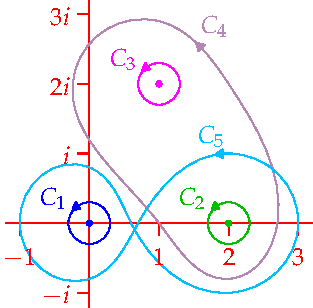
\includegraphics{res1}
\end{minipage}\medbreak
since the latter three integrands are analytic on and inside $C_1$. Similarly,
\begin{gather*}
%\oint_{C_0}f(z)\,\dz=6\pi i,\qquad 
\oint_{C_2}f(z)\,\dz=5i\oint_{C_2}\frac{\dz}{z-2}=-10\pi,\qquad
\oint_{C_3}f(z)\,\dz = \oint_{C_3}\frac{\dz}{z-1-2i}=2\pi i
\end{gather*}
More interesting are the curves $C_4$ and $C_5$. Since $f(z)$ is analytic on and between $C_4$ and $C_2/C_3$, Cauchy--Goursat tells us that
\[\oint_{C_4}f(z)\,\dz=\oint_{C_2}f(z)\,\dz+\oint_{C_3}f(z)\,\dz=2\pi(i-5)\]
$C_5$ appears a little trickier, though it becomes easy once you visualize it as \emph{two} contours: the first encircles $z_2$ \emph{counter-clockwise} while the second passes \emph{clockwise} around $z_1$. We conclude that
\[\int_{C_5}f(z)\,\dz=\oint_{C_2}f(z)\,\dz-\oint_{C_1}f(z)\,\dz=-2\pi(5+3i)\]
\end{example}

The example suggests that the value of any integral round a simple closed contour can be evaluated as a linear combination
\[\int_C f(z)\,\dz=\lambda_1\oint_{C_1}f+\lambda_2\oint_{C_2}f+\lambda_3\oint_{C_3}f\]
where $\lambda_k$ denotes the number of times $C$ orbits $z_k$ in a counter-clockwise direction.\smallbreak 

To properly develop this idea, we need a little formality.\goodbreak

\boldsubsubsection{Isolated Singularities and their Types}

\begin{defn}{}{isolated}
Suppose $f(z)$ is analytic on an punctured disk $0<\nm{z-z_0}<R$ of a point $z_0$, but not at $z_0$ itself. We call $z_0$ an \emph{isolated singularity} of $f(z)$.\par
\begin{minipage}[t]{0.75\linewidth}\vspace{-2pt}
By Laurent's Theorem, $f(z)$ equals its Laurent series on this domain:
\[f(z)=\sum_{n=-\infty}^\infty a_n(z-z_0)^n\quad \text{where}\quad a_n=\frac 1{2\pi i}\oint_C\frac{f(z)}{(z-z_0)^{n+1}}\,\dz\]
and $C$ is any simple closed contour encircling $z_0$. The \emph{residue} of $f(z)$ at $z_0$ is the coefficient
\[\Resl{z=z_0}f(z)=a_{-1}=\frac 1{2\pi i}\oint_C f(z)\,\dz\]
\end{minipage}\begin{minipage}[t]{0.25\linewidth}\vspace{-15pt}
\flushright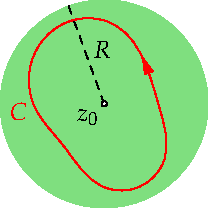
\includegraphics{isolatedsing}
\end{minipage}\medbreak
The type of isolated singularity is determined by the structure of the Laurent series:
\begin{description}
	\item[\normalfont\emph{Removable Singularity}] The Laurent series is a Taylor series. There are no negative powers; the series, and $f(z)$, may be extended analytically to $z_0$. 
	\item[\normalfont{\emph{Pole of order $m$}}] The highest negative power in the Laurent series is $(z-z_0)^{-m}$. A pole of order 1 is typically called a \emph{simple pole.}
	\item[\normalfont\emph{Essential Singularity}] The Laurent series has infinitely many many non-zero negative terms.
\end{description}
% We may also consider the point at $\infty$ to be an isolated singularity, provided $f(z)$ is analytic for all large $z$: i.e.\ when $\nm z>R$.
\end{defn}


\begin{examples}{}{res2}
\hangindent\leftmargini
\textup{1.} \ The series $f(z)=\sum\limits_{n=0}^\infty 3^{-n}(z-2i)^n$ defined on the punctured disk $0<\nm{z-2i}<3$ has a removable singularity at $z_0=2i$ with residue $\smash{\Res\limits_{z=2i}f(z)=0}$. Indeed the function is a geometric series and thus equals
  \[f(z)=\frac 1{1-\frac{z-2i}3}=\frac 3{3+2i-z}\]
  on the punctured disk. Certainly this extends analytically to $f(2i)=1$.
\begin{enumerate}\setcounter{enumi}{1}
  \item (Example \ref{ex:res1})\quad The function $f(z)=\frac 3{z}+\frac 1{z^2}+\frac{5i}{z-2}+\frac 1{z-1-2i}$ is analytic on the punctured disk $0<\nm{z}<0.3$ (inside the circle $C_0$). Since $\frac{5i}{z-2}+\frac 1{z-1-2i}$ is also analytic at zero, the Laurent series of $f(z)$ has the form
  \[f(z)=\frac 3{z}+\frac 1{z^2}+\sum_{n=0}^\infty a_nz^n\]
  We conclude that $f(z)$ has a pole of order 2 at $z_0=0$ and residue $\smash{\Res\limits_{z=0}f(z)=3}$. Similarly, $f(z)$ has simple poles (order 1) at $z_1=2$ and $z_2=1+2i$ with
  \[\Resl{z=2}f(z)=5i,\qquad\Resl{z=1+2i}f(z)=1\]
  	
  \item $\displaystyle e^{1/z}=\sum\limits_{n=0}^\infty\frac{z^{-n}}{n!}=1+\frac 1z+\frac 1{2z^2}+\cdots$ has an essential singularity at zero with $\Res\limits_{z=0}e^{1/z}=1$.
\end{enumerate}
\end{examples}


%In our motivating example (\ref{ex:res1}), we essentially saw that residues can be summed. More generally we have the following key result. 

\begin{thm}[lower separated=false, sidebyside, sidebyside align=top seam, sidebyside gap=0pt, righthand width=0.3\linewidth]{Cauchy's Residue Theorem}{}
If $f(z)$ is analytic on and inside a simple closed $C$, except at finitely many singular points $z_1,\ldots,z_n$, then
\[\oint_Cf(z)\,\dz=2\pi i\sum_{k=1}^n\Resl{z=z_k}f(z)\]
More generally, if $C$ is closed and orbits the point $z_k$ counter-clockwise $w_k$ times (the \emph{winding number}), then
\[\int_Cf(z)\,\dz=2\pi i\sum_{k=1}^nw_k\Resl{z=z_k}f(z)\]
\tcblower
\flushright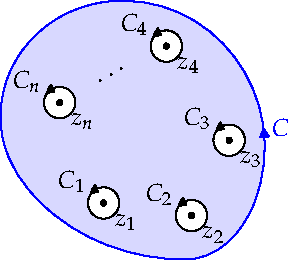
\includegraphics{res2}
\end{thm}


\begin{proof}[Proof. (Simple case)]
Center a small circle $C_k$ at each $z_k$ such that no other singularities lie on or inside $C_k$. Now apply Cauchy--Goursat to the domain on and between $C$ and $C_1\cup\cdots\cup C_n$.
\end{proof}

\begin{examples}{}{res3}
Let $C$ be the circle with radius 4 centered at the origin and $E$ the green curve drawn.

\begin{enumerate}
  \item The function $f(z)=\frac{3(1+iz)}{z(z-3i)}$ has simple poles at $z_1=0$ and $z_2=3i$. There are several ways to compute the residues and thus the integrals $\oint_Cf(z)\dz$ and $\oint_Ef(z)\dz$.\smallbreak
\begin{minipage}[t]{0.67\linewidth}\vspace{-10pt}
\emph{Partial Fractions}\quad For \emph{this} example, this is very easy.
\begin{align*}
f(z)=\frac iz+\frac{2i}{z-3i} &\implies \Resl{z=0} f(z)=i,\quad \Resl{z=3i} f(z)=2i\\
&\implies \oint_Cf(z)\,\dz=2\pi i(i+2i)=-6\pi
\end{align*}
The curve $E$ is the union of three closed curves; twice \emph{clockwise} around $z_1$ and once  \emph{counter-clockwise} around $z_2$. Therefore
\[\int_Ef(z)\,\dz=2\pi i\left[-2\Resl{z=0} f(z)+\Resl{z=3i}f(z)\right] =0\]
\end{minipage}
\begin{minipage}[t]{0.32\linewidth}\vspace{0pt}
\flushright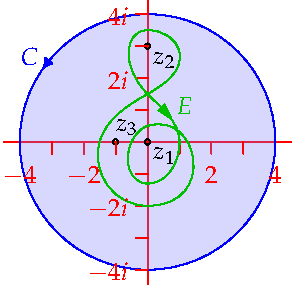
\includegraphics{res3}
\end{minipage}\medbreak

\emph{Laurent series}\quad Remember that we only need the $z^{-1}$ terms for the \textcolor{red}{residues}!
\begin{gather*}
  \frac{3(1+iz)}{z(z-3i)}=\frac{i-z}{z(1-\frac{iz}3)}=\left(iz^{-1}-1\right)\sum_{n=0}^\infty\left(\frac{iz}3\right)^n =\frac{\textcolor{red}{i}}z+\text{power series}\\
  \frac{3(1+iz)}{z(z-3i)}=\frac{z-3i+2i}{(1+\frac{z-3i}{3i})(z-3i)}=\left(\frac{2i}{z-3i}+1\right)\sum_{n=0}^\infty\left(\frac{3i-z}{3i}\right)^n =\frac{\textcolor{red}{2i}}{z-3i}+\text{power series}
  \end{gather*}
  
\emph{Cauchy's formula}\quad Let $C_k$ be a small circle around $z_k$, then
  \begin{gather*}
  \Res_{z=0}f(z)=\frac 1{2\pi i}\oint_{C_1}f(z)\,\dz =\frac 1{2\pi i}\oint_{C_1}\frac{3(1+iz)}{z(z-3i)}\,\dz = \frac{3(1+iz)}{z-3i}\bigg|_{z=0}=i\\
  \Res_{z=3i}f(z)=\frac 1{2\pi i}\oint_{C_2}f(z)\,\dz =\frac 1{2\pi i}\oint_{C_2}\frac{3(1+iz)}{z(z-3i)}\,\dz = \frac{3(1+iz)}{z}\bigg|_{z=3i}=2i
  \end{gather*}
  We'll revisit this last approach in the next section.
  \goodbreak
  
  \item Plainly $f(z)=z^2\sin\frac 1z$ has one isolated singularity at the origin. Using the Maclaurin series for $\sin z$, we see that this is an essential singularity, and can easily evaluate the required integrals:
  \[z^2\sin\frac 1z=\sum_{n=0}^\infty \frac{(-1)^n}{(2n+1)!}z^{1-2n} \implies \oint_Cz^2\sin\frac 1z\,\dz=2\pi i\Resl{z=0}\left(z^2\sin\frac 1z\right) =-\frac{\pi i}3\]
  Since $E$ loops twice \emph{clockwise} around the origin, we obtain
  \[\int_Ez^2\sin\frac 1z\,\dz=2\pi i\cdot (-2)\Resl{z=0}\left(z^2\sin\frac 1z\right) =\frac{2\pi i}3\]  

	\item The function $f(z)=3e^{1/z}+\frac 4{z-7i}+\frac{2i}{z+1}$ has an essential singularity at the origin and simple poles at $-1$ and $7i$. Since the last of these lies \emph{outside} the curves $C,E$, it does not contribute to either integral. Moreover, note that $E$ loops \emph{twice} clockwise around the origin and \emph{once} clockwise around $z_3=-1$. We therefore have
  \begin{gather*}
  \oint_Cf(z)\,\dz=2\pi i\left(\Resl{z=0}3e^{1/z}+\Resl{z=-1} \frac{2i}{z+1}\right)=2\pi i(3+2i)\\
  \oint_Ef(z)\,\dz=2\pi i\left(-2\Resl{z=0}3e^{1/z}-\Resl{z=-1} \frac{2i}{z+1}\right)=2\pi i(-6-2i)=4\pi(1-3i)
  \end{gather*}
\end{enumerate}
\end{examples}

\goodbreak

\boldsubsubsection{Non-isolated Singularities}

Consider the converse of Definition \ref{defn:isolated}: a singularity $z_0$ is non-isolated if \emph{every} punctured disk $0<\nm{z-z_0}<R$ contains at least one point where $f(z)$ is non-analytic. Necessarily this requires $f(z)$ to be non-analytic at infinitely many points. Non-isolated singularities typically appear in two flavors.

\begin{examples}{}{}
\hangindent\leftmargini
\textup{1.} \ The function $f(z)=\bigl(\polar{2\pi i}z-1\bigr)^{-1}$ has singularities at $z_0=0$ and whenever $z_n=\frac 1n$ for each non-zero integer $n$. Each of the \textcolor{blue}{non-zero singularities} is isolated (e.g.\ choose \textcolor{blue}{$R_n=\frac 1{(\nm n+1)^2}$}). The remaining \textcolor{Green}{\emph{limit point}} $z_0=0$ is a non-isolated singularity: for any $R>0$, the \textcolor{Green}{punctured disk $0<\nm z<R$} contains \textcolor{blue}{non-zero singularities}.
\begin{center}
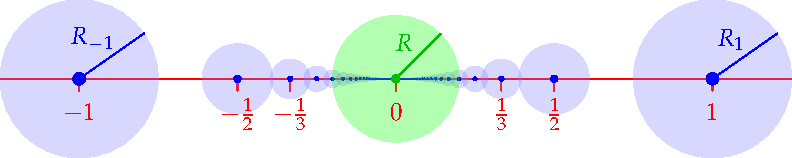
\includegraphics{sing1}
\end{center}

\begin{enumerate}\setcounter{enumi}{1}
\begin{minipage}[t]{0.7\linewidth}\vspace{0pt}
  \item The function $f(z)=\sqrt z$ has \textcolor{Green}{\emph{branch point}} $z_0=0$. For $f$ to be analytic, we need to make a branch cut: for instance, the principal value of $\sqrt z$ has the \textcolor{blue}{non-positive real axis} as a branch cut.\par
  Since any \textcolor{Green}{domain $0<\nm z<R$} contains other points of the \textcolor{blue}{branch cut} (where $f$ is non-analytic), it follows that a branch point is a non-isolated singularity \emph{for any branch} of $f$.\par
\end{minipage}\begin{minipage}[t]{0.3\linewidth}\vspace{10pt}
\flushright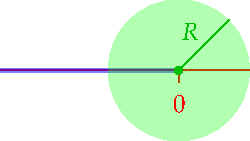
\includegraphics{sing2}
\end{minipage}
\end{enumerate}
\end{examples}

\goodbreak

\begin{exercises*}
\hangindent\leftmargini
\textup{1.} \ For each of the following types of singularity, what, if anything, can you say about the value of the residue $\Res\limits_{z=z_0}f(z)$? Choose from `Equals zero,' `Non-zero,' `No restriction'.\vspace{-5pt}
\begin{enumerate}\setcounter{enumi}{1}
  \item[]\begin{enumerate}
	  \item Removable singularity.
	  \item Simple pole.
	  \item Pole of order $m\ge 2$.
	  \item Essential singularity.
	\end{enumerate}
	
  \item	Find the residue at $z=0$ of each function:
  \begin{enumerate}
    \item $\dfrac 1{z+3z^2}$\qquad (b)\ \ $\displaystyle z\cos\frac 1z$\qquad (c) \ \ $\dfrac{z-\sin z}{z}$
	\end{enumerate}
	
	\item Let $C$ be the circle $\nm z=3$. Evaluate the integrals using Cauchy's residue theorem:
  \begin{enumerate}
    \item $\displaystyle\oint_C\frac{e^{-z}}{z^2}\,\dz$\qquad (b)\ \ $\displaystyle\oint_C\frac{e^{-z}}{(z-1)^2}\,\dz$\qquad (c) \ \ $\displaystyle\oint_Cz^2e^{1/z}\,\dz$\qquad (d)\ \ $\displaystyle\oint_C\frac{z+1}{z^2-2z}\,\dz$
	\end{enumerate}
	
	\item Suppose a closed contour $C$ loops twice counter-clockwise around $z=i$ and three times clockwise around $z=2$. Use residues to compute the integral
	\[\int_C\frac{z+3}{(z-2)^2(z-i)}\dz\]
	
	\item Identify the type of singular point of each of the following functions and determine the residue:
	\begin{enumerate}
	  \item $\dfrac{1-\cosh z}{z^3}$\qquad (b)\ \ $\dfrac{1-e^{2z}}{z^4}$\qquad (c)\ \ $\dfrac{e^{2z}}{(z-1)^2}$
	\end{enumerate}
	
	\item Suppose $f(z)$ is analytic at $z_0$ and define $g(z)=(z-z_0)^{-1}f(z)$. Prove:
	\begin{enumerate}
	  \item If $f(z_0)\neq 0$, then $z_0$ is a simple pole of $g(z)$ with $\Res\limits_{z=z_0}g(z)=f(z_0)$;
	  
	  \item If $f(z_0)= 0$, then $z_0$ is a removable singularity of $g(z)$.
	\end{enumerate}

	
	\item Let $P(z)$ and $Q(z)$ be polynomials whose degrees satisfy $2+\deg P\le \deg Q$ and assume $C$ is a simple closed contour such that all zeros of $Q(z)$ lie interior to $C$.
	\begin{enumerate}
	  \item Prove that $\displaystyle\oint_C\frac{P(z)}{Q(z)}\,\dz=0$\par
		(\emph{Hint: Try the substitution $w=\frac 1z$})
		
		\item What can you conclude if $\deg Q=\deg P+1$?
	\end{enumerate}
	
% 	\item A function which is analytic on an infinite annulus $\nm{z}>R$ is said to have an isolated singularity at $\infty$ and \emph{residue at infinity} defined by
% 	\[\Res_{z=\infty}f(z):=-\Res_{z=0}\left(z^{-2}f(z^{-1})\right)\]
% 	It follows that, on this domain, we have a Laurent series
% 	\[f(z)=\sum_{n=-\infty}^\infty a_nz^n\]
% 	\begin{enumerate}
% 	  \item What properties do you think this series should have if we were to describe the singularity at $\infty$ to be:
% 	  \begin{enumerate}
% 	    \item Removable?\qquad ii.\ \ A pole of order $m$?\qquad iii.\ \ Essential?
% 	  \end{enumerate}
% 
% 	  \item The \emph{residue at $\infty$} of the above function is defined to be $\Resl{z=\infty}f(z)=-a_{-1}$. For example $\Resl{z=\infty}\frac{z^2+1}{z^3}=-1$. Prove that:
% 	 	\begin{enumerate}
% 	    \item $\Resl{z=\infty}f(z)=\int$
% 
% 	    \item Removable?
% 	  \end{enumerate}
% 	\end{enumerate}
	


\end{enumerate}
\end{exercises*}
\clearpage


\subsection{Poles \& Zeros}

Recall Example \ref{ex:res3} where we used Cauchy's integral formula as one of the methods for computing a residue. If the order of a pole is known, this approach is often fairly efficient.

\begin{thm}{}{polesimple}
A function $f(z)$ has a pole of order $m$ at $z_0$ if and only if $f(z)=(z-z_0)^{-m}\phi(z)$ where $\phi(z)$ is \emph{analytic} at $z_0$ and $\phi(z_0)\neq 0$. In such a case,
\footnote{This formula works even if $\phi(z_0)=0$; you only need $\phi(z)$ analytic and \emph{non-constant} at $z_0$: a naïve application means you won't know the order of the pole and you'll have to differentiate more times than necessary!}
\[f(z)=(z-z_0)^{-m}\sum_{n=0}^\infty \frac{\phi^{(n)}(z_0)}{n!}(z-z_0)^n \implies \Res_{z=z_0}f(z)=\frac 1{(m-1)!}\phi^{(m-1)}(z_0)\]
This specializes to $\Res\limits_{z=z_0}f(z)=\phi(z_0)$ for a simple pole.
\end{thm}

\begin{examples}{}{polecalceasy}
\hangindent\leftmargini
\textup{1.} \ (Example \ref{ex:res3})\quad Write \smash[b]{$\displaystyle f(z)=\frac{3(1+iz)}{z(z-3i)}=\frac{\phi_1(z)}z =\frac{\phi_2(z)}{z-3i}$} and verify:
\begin{enumerate}\setcounter{enumi}{1}
  \item[]\emph{Simple pole at $z_1=0$}:\quad $\phi_1(z)=\frac{3(1+iz)}{z-3i}$ is analytic, and $\phi_1(0)=\frac 3{-3i}=i=\Res\limits_{z=0}f(z)$\smallbreak
\emph{Simple pole at $z_2=3i$}:\quad $\phi_2(z)=\frac{3(1+iz)}{z}$ is analytic, and $\phi_2(3i)=\frac{3(1-3)}{3i}=2i=\Res\limits_{z=3i}f(z)$
  
  \item Write {$\displaystyle f(z)=\frac{1-2iz}{(z-1)(z-2i)^3}=\frac{\phi_1(z)}{z-1} =\frac{\phi_2(z)}{(z-2i)^{3}}$} and compute:\smallbreak
	\emph{Simple pole at $z_1=1$}:\quad $\phi_1(z)=\frac{1-2iz}{(z-2i)^3}$ is analytic and non-zero at $z_1=1$. It follows that
    \[\Resl{z=1}f(z)=\phi_1(1)=\frac{1-2i}{(1-2i)^3}=\frac 1{(1-2i)^2}=\frac{4i-3}{25}\]
  \emph{Pole of order three at $z_2=2i$}:\quad $\phi_2(z)=\frac{1-2iz}{z-1}=-2i+\frac{1-2i}{z-1}$ is analytic and non-zero at $2i$, and
    \[\Resl{z=2i}f(z)=\frac 1{(3-1)!}\phi_2''(2i)=\frac{1-2i}{(z-1)^3}\bigg|_{z=2i}=\frac{-1}{(2i-1)^2}=\frac{3-4i}{25}\]
\end{enumerate}
\end{examples}

\begin{proof}
($\Rightarrow$)\quad By Laurent's Theorem, $f(z)$ equals its Laurent series. It moreover has a pole of order $m$ at $z_0$ if and only if
\[f(z)=\sum_{n=-m}^\infty a_n(z-z_0)^n =(z-z_0)^{-m}\sum_{n=0}^\infty a_{n-m}(z-z_0)^n\ \text{ where }\ a_{-m}\neq 0\tag{$\ast$}\]
Plainly $\phi(z):=\sum\limits_{n=0}^\infty a_{n-m}(z-z_0)^n$ is analytic at $z_0$ and satisfies $\phi(z_0)=a_{m-n}\neq 0$.\smallbreak
($\Leftarrow$)\quad Taylor's Theorem says that $\phi(z)$ equals its Taylor series $\sum\limits_{n=0}^\infty a_{n-m}(z-z_0)^n$, whence (uniqueness of representation) $(\ast)$ is \emph{the} Laurent series of $f(z)$ and $f(z)$ has a pole of order $m$.
%\medbreak
% The residue formula is immediate from the Taylor series of $\phi(z)$:
% \[f(z)=(z-z_0)^{-m}\sum_{n=0}^\infty \frac{\phi^{(n)}(z_0)}{n!}(z-z_0)^n \implies \Res_{z=z_0}f(z)=\frac 1{(m-1)!}\phi^{(m-1)}(z_0)\tag*{\qedhere}\]
% The residue formula comes from applying Cauchy's integral formula to a small circle around $z_0$:
% \[a_{-1}=\frac 1{2\pi i}\oint_Cf(z)\,\dz=\frac 1{(m-1)!}\cdot\frac{(m-1)!}{2\pi i}\oint_C\frac{\phi(z)}{(z-z_0)^m}\,\dz =\frac 1{(m-1)!}\phi^{(m-1)}(z_0)\tag*{\qedhere}\]
\end{proof}

As the examples show, the method is very effective when $f(z)$ is rational with low-order poles; as a bonus, it saves us from partial fractions! Its utility is more variable for other functions\ldots

\begin{examples}{}{residuesdiffmethod}
\hangindent\leftmargini
\textup{1.} \ Taking $\phi(z)=\frac{e^z}{z+1}$ shows that the non-rational function
\[f(z)=\frac{e^z}{(z-1)^2(z+1)}=\frac{\phi(z)}{(z-1)^2}\]
has a pole of order two at $z_0=1$ and moreover that
\[\Resl{z=1}f(z)=\frac 1{(2-1)!}\phi'(1)=\frac{(z+1)e^z-e^z}{(z+1)^2}\bigg|_{z=1} =\frac 14e\]
\begin{enumerate}\setcounter{enumi}{1}
  \item\label{ex:residuesdiffmethod2} Don't let the denominator fool you! At first glance we appear to have a pole of order \emph{six}: 
	\[f(z)=\frac{6\sin z-6z+z^3}{z^6}=\frac{\smash[t]{\widetilde\phi(z)}}{z^6}\overset{\text{??}}{\implies} \Resl{z=0}f(z)=\frac 1{5!}\widetilde\phi^{(5)}(0)=\frac 6{120}=\frac 1{20}\]
	However, if we apply the Maclaurin series for sine, we instead find a \emph{simple pole}:
	\begin{align*}
  f(z)&=\frac 1{z^6}\left(6\sum_{n=0}^\infty\frac{(-1)^n}{(2n+1)!}z^{2n+1}-6z+z^3\right)=z^{-6}\sum_{n=2}^\infty\frac{6(-1)^n}{(2n+1)!}z^{2n+1}\\
  &=z^{-1}\textcolor{Green}{\sum_{m=0}^\infty\frac{6(-1)^m}{(2m+5)!}z^{2m}}=\frac 1{20z}+\frac 1{840}+\cdots\implies \Resl{z=0}f(z)=\frac 1{20}
  \end{align*}
  Even though the residue was correct, our original $\smash[t]{\widetilde\phi}$ was wrong ($\smash[t]{\widetilde\phi}(0)\neq 0$). The correct function is the series \textcolor{Green}{$\phi(z)=6\sum\limits_{m=0}^\infty\frac{(-1)^m}{(2m+5)!}z^{2m}$}.
\end{enumerate}
\end{examples}


\boldsubsubsection{Zeros of Analytic Functions}

It turns out that poles and zeros of analytic functions are intimately related. We start by mirroring Definition \ref{defn:isolated} and Theorem \ref{thm:polesimple}.

\begin{defn}{}{}
Suppose $f(z)$ is analytic at $z_0$ and $f(z_0)=0$. We say that $z_0$ is a \emph{zero of order $m$} if $f^{(m)}(z_0)$ is the first \emph{non-zero} derivative. We refer to a \emph{simple zero} when $m=1$.\smallbreak
A zero $z_0$ is \emph{isolated} if it has some neighborhood with no other zeros:
\[\exists R>0\text{ such that }0<\nm{z-z_0}<R\implies f(z)\neq 0\]
\end{defn}

We are used to the idea of polynomial having a zero $z_0$ if and only if we can factorize out $z-z_0$. The tight link-up with Taylor series makes essentially this observation hold for \emph{any} analytic function!


\begin{lemm}{}{zerofactor}
A function $f(z)$ has a zero $z_0$ of order $m$ if and only if $f(z)=(z-z_0)^m\psi(z)$ where $\psi(z)$ is analytic at $z_0$ and $\psi(z_0)\neq 0$. Indeed, on some disk $\nm{z-z_0}<R_0$,
\[f(z)=\sum\limits_{n=m}^\infty\frac{f^{(n)}(z_0)}{n!}(z-z_0)^{n} =(z-z_0)^{m}\psi(z)\]
\end{lemm}
\goodbreak



\begin{examples}{}{}
\hangindent\leftmargini
\textup{1.} \ $f(z)=z^4(z-2i)^{10}=z^4\psi_1(z)=(z-2i)^{10}\psi_2(z)$ has two zeros:
\begin{enumerate}\setcounter{enumi}{1}
  \item[]\emph{Order four at $z_1=0$}:\quad $\psi_1(z)=(z-2i)^{10}\implies\psi_1(0)=-1024\neq 0$.\smallbreak
\emph{Order ten at $z_2=2i$}:\quad $\psi_2(z)=z^4\implies\psi_2(2i)=16\neq 0$.

	\item $g(z)=17(z-4i)^3\cos z$ has a zero of order three at $4i$, and simple zeros at each half-integer multiple $\left(\frac 12\pm k\right)\pi$ of $\pi$. For instance
	\begin{align*}
	g(z)&=17(z-4i)^3\cos\left(z-\frac\pi 2+\frac\pi 2\right)= -17(z-4i)^3\sin\left(z-\frac\pi 2\right)\\
	&=-17(z-4i)^3\sum_{n=0}^\infty\frac{(-1)^n}{(2n+1)!}\left(z-\frac\pi 2\right)^{2n+1}\\
	&=\left(z-\frac\pi 2\right)\left[-17(z-4i)^3\sum_{n=0}^\infty\frac{(-1)^n}{(2n+1)!}\left(z-\frac\pi 2\right)^{2n}\right] =\left(z-\frac\pi 2\right)\psi(z)
	\end{align*}
\end{enumerate}
\end{examples}


The examples are typical: just as with singularities, the typical arrangement is for a zero of an analytic function to be \emph{isolated.} Indeed, analytic functions with non-isolated zeros are very boring\ldots

\begin{thm}{}{isolatedzero}
Let $z_0$ be a zero of an analytic function $f(z)$. The following are equivalent:
\begin{enumerate}
  \item $f(z)$ is non-zero at some point of every neighborhood $\nm{z-z_0}<\epsilon$ of $z_0$.
  \item $z_0$ is a zero of some positive order $m$.
  \item $z_0$ is an isolated zero.
\end{enumerate}
\end{thm}

The distinction between conditions 1 and 3 is important: the first is weaker and the the equivalence is \emph{false} for non-analytic functions. For example, at $z_0=0$ the non-analytic function $f(z)=z+\cl z=2x$ satisfies condition 1 but not 3 (e.g.\ $f(\frac\epsilon 2)\neq 0$). There is something to prove here!

\begin{proof}
\begin{description}
  \item[$(1\Rightarrow 2)$]\quad The Taylor series of $f(z)$ is non-zero, else $f(z)$ would be zero on some disk $\nm{z-z_0}<\epsilon$. There must therefore be some minimum $m\in\N$ such that $f^{(m)}(z_0)\neq 0$, whence $z_0$ is a zero of order $m$.
	\item[$(2\Rightarrow 3)$]\quad $f(z)=(z-z_0)^m\psi(z)$ where $\psi(z)$ is analytic and $\psi(z_0)\neq 0$. Since $\psi(z)$ is continuous, it is non-zero on some disk $\nm{z-z_0}<\epsilon$, and so also is $f(z)$. We conclude that $z_0$ is an isolated zero.
	\item[$(3\Rightarrow 1)$]\quad This is trivial.\qedhere
\end{description}
\end{proof}

\begin{cor}{}{}
If $f(z)$ is analytic on a connected open domain $D$ containing $z_0$, and $f(z)=0$ at each point of some contour $C$ containing $z_0$, then $f(z)\equiv 0$ on $D$.
\end{cor}
 
\begin{proof}
This is the negation of the situation in the Theorem: plainly $z_0$ is not isolated and so $f(z)\equiv 0$ on some disk centered on $z_0$. The usual patching argument extends this to $D$.
\end{proof}

This essentially proves the result regarding unique analytic continuations from earlier in the course.

\goodbreak

\boldsubsubsection{Reciprocals switch poles and zeros}

It seems intuitive that we can turn poles into zeros just by flipping a function upside down.

\begin{thm}{}{polezeroreverse}
Let $f(z)$ be analytic at $z_0$ and $g(z)=\frac 1{f(z)}$. Then, at $z_0$,\vspace{-2pt}
\[f(z)\text{ has a zero of order }m\iff g(z)\text{ has a pole of order }m\] 
\end{thm}

The proof is an easy exercise in combining Theorem \ref{thm:polesimple} and Lemma \ref{lemm:zerofactor}.\smallbreak

% \begin{proof}
% Write $f(z)=(z-z_0)^m\psi(z)$ and $g(z)=(z-z_0)^{-m}\phi(z)$ where $\phi(z)=\frac 1{\psi(z)}$. Then\vspace{-2pt}
% \[\psi(z)\text{ is analytic and non-zero at }z_0\iff \phi(z)\text{ is also}\tag*{\qedhere}\]
% \end{proof}

This approach yields a very quick method for computing residues of functions with \emph{simple poles,} and is particularly useful which a function is multi-valued.

\begin{cor}{}{easyres}
Suppose $p,q$ are analytic at $z_0$ such that $f(z)=\frac{p(z)}{q(z)}=\frac{p(z)}{(z-z_0)\psi(z)}$ has a simple pole at $z_0$. Plainly $q'(z_0)=\psi(z_0)$, from which\vspace{-2pt}
\[\Resl{z=z_0}\frac{p(z)}{q(z)} =\frac{p(z_0)}{q'(z_0)}\]
\end{cor}

\begin{examples}{}{}
\hangindent\leftmargini
\textup{1.} \ The function $f(z)=\frac{p(z)}{q(z)}=\frac{(z^2+1)^2}{z-3}=\frac{(z-i)^2(z+i)^2}{z-3}$ has zeros of order two at $\pm i$ and a simple pole at $z=3$. The reciprocal has the reverse arrangement: poles of order two at $\pm i$ and a simple zero at $3$. Moreover,
  \[\Resl{z=3}f(z)=\frac{p(3)}{q'(3)}=\frac{(3^2+1)^2}{1}=100\]
\begin{enumerate}\setcounter{enumi}{1}
  \item The function $g(z)=\frac{p(z)}{q(z)}=\frac{\sin z}{z^2+4} =\frac{\sin z}{(z-2i)(z+2i)}$ has simple poles at $\pm 2i$  with 
  \[\Resl{z=2i}f(z)=\Resl{z=-2i}f(z)=\frac{p(\pm 2)}{q'(\pm 2)}=\frac{\sin 2i}{4i}=\frac 18(e^2-e^{-2}) =\frac 14\sinh 2\]
  The reciprocal has simple poles at $z=n\pi$ for every $n\in\Z$: moreover
  \[\Resl{z=n\pi}\frac 1{f(z)}=\frac{q(n\pi)}{p'(n\pi)}=\frac{n^2\pi^2+4}{\cos n\pi}= (-1)^n(n^2\pi^2+4)\]
  
  \item Since $q(z)=e^{2z}-1=\sum\limits_{n=1}^\infty\frac{2^nz^n}{n!}=z\sum\limits_{n=0}^\infty\frac{2^nz^n}{(n+1)!}$ has a simple zero at $z=0$, we see that
  \[f(z)=\frac{\sqrt{z+4i}}{(z+i)^2\Log(z+2)(e^{2z}-1)}=\frac{p(z)}{q(z)}\]
  has a simple pole at $z=0$ (we use the principal value of $\sqrt{z+4i}$). Moreover
  \[\Resl{z=0}f(z)=\frac{p(0)}{q'(0)}=\frac{\polar{i\pi}4}{\ln 2} =\frac{1+i}{\sqrt 2\ln 2}\]
  We could instead have chosen $q(z)=(z+i)^2\Log(z+2)(e^{2z}-1)$, but the differentiation would have been much worse!
\end{enumerate}
\end{examples}
\goodbreak

\boldsubsubsection{Counting Poles and Zeros}

\begin{defn}{}{}
A function $f$ is \emph{meromorphic} on a domain $D$ if it is analytic except at isolated \emph{poles.} That is, $f$ cannot have essential (or removable) singularities. 
\end{defn}

\begin{thm}{}{}
Suppose $C$ is a positively oriented closed contour. If $f$ is meromorphic on and inside $C$, then
\[\frac 1{2\pi i}\oint_C\frac{f'(z)}{f(z)}\,\dz =Z-P\]
where $Z$ and $P$ are the number of zeros and poles of $f$ inside $C$, counted up to multiplicity.
\end{thm}

\begin{example}{}{}
Consider, $f(z)=\frac{(z-i)^2\sin z}{(z-5)^4}$ where $C$ is a large circle surrounding the points 0, $i$ and 5. Plainly $Z=2+1=3$ and $P=4$. By an unpleasant application of the quotient rule (or better using logarithms, just be careful!), we obtain
\[\frac 1{2\pi i}\oint_C\frac{f'(z)}{f(z)}\,\dz =\frac 1{2\pi i}\oint_C\frac 2{z-i}+\frac{\cos z}{\sin z}-\frac 4{z-5}\,\dz =2+\cos 0-4=-1 =Z-P\]
\end{example}

\begin{proof}
If $f$ has a zero of order $m$ at $z=z_k$, then $f(z)=(z-z_k)^m\psi(z)$ on and inside a some small circle $C_k$ centered at $z_k$, where $\psi(z)$ is analytic and \emph{non-zero.} But then
\begin{align*}
\oint_{C_k}\frac{f'(z)}{f(z)}\,\dz&=\oint_{C_k}\frac{m(z-z_0)^{m-1}\psi(z)+(z-z_0)^m\psi'(z)}{(z-z_0)^m\psi(z)} \,\dz= \oint_{C_k}\frac m{z-z_0}+\frac{\psi'(z)}{\psi(z)} \,\dz\\
&=2\pi im
\end{align*}
Similarly, if $f$ has a pole of order $m$, then we repeat with $f(z)=(z-z_k)^{-m}\phi(z)$ to obtain
\begin{align*}
\oint_{C_k}\frac{f'(z)}{f(z)}\,\dz&=\oint_{C_k}\frac{-m(z-z_0)^{-m-1}\phi(z)+(z-z_0)^{-m}\phi'(z)}{(z-z_0)^{-m}\phi(z)} \,\dz= \oint_{C_k}-\frac m{z-z_0}+\frac{\phi'(z)}{\phi(z)} \,\dz\\
&=-2\pi im
\end{align*}
Cauchy's residue theorem completes the proof.
\end{proof}

\boldsubsubsection{Properties of Singularities}

We finish by considering some equivalent conditions for the various types of singularities.

\begin{thm}{Removable Singularities}{}
Suppose $f(z)$ has an isolated singularity at $z_0$ (and is therefore analytic on a punctured disk $0<\nm z<R$). The following are equivalent:
\begin{enumerate}
	\item The singularity is removable.
	\item \smash[b]{$\lim\limits_{z\to z_0}f(z)$} exists and is finite.
	\item $f(z)$ is bounded on some $0<\nm{z-z_0}<\delta$.
\end{enumerate}
\end{thm}

\begin{proof}
For simplicity, suppose that $z_0=0$.
\begin{description}
  \item[]($1\Rightarrow 2$)\quad \smash[b]{$f(z)=\sum\limits_{n=0}^\infty a_nz^n$} on $0<\nm z<R$, whence \smash[b]{$\lim\limits_{z\to 0}f(z)=a_0$}.
	\item[]($2\Rightarrow 3$)\quad This is almost tautological but it bears repeating: If \smash[b]{$\lim\limits_{z\to 0}f(z)=a_0$} exists and is finite then choose $\epsilon=\nm{a_0}$ in the definition;
	\begin{align*}
	\exists \delta>0\text{ such that }0<\nm z<\delta&\implies \nm{f(z)-a_0}<\nm{a_0}\\
	&\implies \nm{f(z)}=\nm{f(z)-a_0+a_0}\le 2\nm{a_0}
	\end{align*}
	\item[]($3\Rightarrow 1$)\quad Consider
	\[g(z)=\begin{cases}
	z^2f(z)&\text{if }0<z<\delta\\
	0&\text{if }z=0
	\end{cases}\]
	Since $f$ is bounded, we may compute the limit
	\[\lim_{z\to 0}\frac{g(z)-g(0)}{z}=\lim_{z\to 0}zf(z)=0\]
	whence $g(z)$ is differentiable at zero! Since it is already differentiable on the punctured neighborhood $0<\nm z<\min\{\delta,R\}$, it is therefore analytic on the \emph{disk} $\nm z<\min\{\delta,R\}$ and equals its Maclaurin series
	\[g(z)=\sum_{n=0}^\infty b_nz^n\]
	However $g(0)=0=g'(0)\implies b_0=b_1=0$ and so
	\[g(z)=z^2\sum_{n=0}^\infty b_{n-2}z^n\implies f(z)=\sum\limits_{n=0}^\infty b_{n-2}z^n\text { on }0<\nm z<\min\{\delta,R\}\]
	whence $f$ has a removable singularity.\qedhere
\end{description}
\end{proof}

We leave the remaining results as exercises.
\begin{thm}{}{casorati}
Suppose $f$ has an isolated singularity at $z=z_0$.
\begin{enumerate}
  \item $z_0$ is a pole if and only if \smash[b]{$\lim\limits_{z\to z_0}f(z)=\infty$.}
  \item If $z_0$ is essential and $w\in\C\cup\{\infty\}$, then $\exists z_n\to z_0$ such that $f(z_n)\to w$. 
\end{enumerate}
\end{thm}

This second result is the \emph{Casorati--Weierstrass Theorem}; the range of $f(z)$ is \emph{dense} in a neighborhood of an essential singularity. A stronger result is available, through its proof is beyond us.

\begin{thm}{Picard}{}
If $z_0$ is an essential singularity of $f(z)$, then $f(z)$ takes every complex value \emph{except at most one} in any neighborhood of $z_0$.
\end{thm}

\begin{example}{}{}
Let $f(z)=e^{1/z}$ at $z_0=0$. If $w=e^{1/z}$, write $w=re^{i\theta}$ with $0\le \theta<2\pi$, from which
\[e^{\ln r+i\theta}=e^{1/z}\implies \frac 1z=\ln r+i\theta+2\pi in\]
for any integer $n$. If $n>0$, observe that
\[\nm{\frac 1z}=\sqrt{(\ln r)^2+(\theta+2\pi n)^2}>2\pi n\]
whence $\nm z$ can be chosen arbitrarily small. A suitable $z$ thus exists in any punctured disk $0<\nm z<\delta$.
\end{example}



\begin{exercises*}
\hangindent\leftmargini
\textup{1.} \ Determine the order of each pole and its residue.
\begin{enumerate}\setcounter{enumi}{1}
  \item[]\begin{enumerate}
    \item $f(z)=\dfrac{z+1}{z^2+9}$\qquad (b)\ \ $f(z)=\left(\dfrac{z}{2z+1}\right)^3$
  \end{enumerate}
  
  \item Show that:
  \begin{enumerate}
    \item $\Res\limits_{z=-1}\frac{z^{1/4}}{z+1}=\frac{1+i}{\sqrt 2}$ when $\nm z>0$ and $\arg z\in(0,2\pi)$
    
    \item $\Res\limits_{z=i}\frac{\Log z}{(z^2+1)^2}=\frac{\pi+2i}8$
    
    \item $\Res\limits_{z=z_n}\bigl(z\sec z\bigl)=(-1)^{n+1}z_n$, where $z_n=\frac\pi 2+n\pi$ and $n\in\Z$
  \end{enumerate}
  
  \item Find the value of the integral
  \[\oint_C\frac{3z^3+2}{(z-1)(z^2+9)}\,\dz\]
 	when $C$ is each of the circles: (a)\ $\nm{z-2}=2$ and \ (b)\ $\nm z=4$.
  
  \item Let $C$ be the circle $\nm z=2$. Evaluate $\oint_C\tan z\,\dz$.
  
  \item Prove Theorem \ref{thm:polezeroreverse}.
  
  \item Let $f(z)=\left(z\sin\frac\pi z\right)^{-1}$
  \begin{enumerate}
    \item Evaluate $\Res\limits_{z=\frac 1n}f(z)$ for each $n\in\Z$.
    \item Why doesn't $\Res\limits_{z=0}f(z)$ make sense?
  \end{enumerate}
  
	\item Suppose $f(z)$ is analytic and non-constant at $z_0$. Prove that
	\[\exists\epsilon>0\ \text{such that}\ 0<\nm{z-z_0}<\epsilon\implies f(z)\neq f(z_0)\]  

  
  \item Suppose that $C$ is the rectangle whose sides are the lines $x=\pm 2, y=0$ and $y=1$. Prove that
  \[\oint_C\frac{\dz}{(z^2-1)^2+3}=\frac\pi{2\sqrt 2}\]
  (\emph{Hint: the integrand has four simple poles, only two of which lie inside $C$})
  
  \item[]The last two questions are more of a challenge

	\item Prove Theorem \ref{thm:casorati}. For simplicity, assume $z_0=0$.
	\begin{description}  	
  	\item[]\emph{Hint 1: $f(z)$ has a pole if and only if $\frac 1{f(z)}$ has a zero.}
  	\item[]\emph{Hint 2: If no such sequence exists, show that $g(z):=\frac 1{f(z)-w}$ is analytic and bounded.}
	\end{description}
	
	  
  \item Suppose $f(z)$ is analytic on and inside a simple closed curve $C$, and that it has no zeros on $C$. We consider the integral
  \[I=\frac 1{2\pi i}\oint_C\frac{f'(z)}{f(z)}\,\dz\]
  \begin{enumerate}
    \item Explain why $I$ counts the number of zeros (including multiplicity) of $f(z)$ inside $C$.
    \item (Winding number)\quad Explain why $I$ also counts the number times the curve $\gamma=f(C)$ orbits the origin counter-clockwise.\par
    (\emph{Hint: let $w=f(z)$})
    \item (Rouche's Theorem)\quad Suppose that $\nm{g(z)}<\nm{f(z)}$ for all $z\in C$. Prove that the number of zeros of $f+g$ inside $C$ equals that of $f$.\par
    (\emph{Hint: Apply part (a) to the product $f+g=f\cdot(1+\frac gf)$ and consider why the function $1+\frac gf$ has winding number zero})
    \item Since $\nm{4z^3}>\nm{z^{22}+2i}$ on the circle $\nm z=1$, how many solutions (up to multiplicity) are there to the equation $z^{22}+4z^3+2i=0$ on the domain $\nm z<1$?
  \end{enumerate}

\end{enumerate}
\end{exercises*}
\clearpage

\subsection{Improper Integrals}

We describe a natural application of residues to the evaluation of certain \emph{real} improper integrals. We start with an alternative definition of improper integral more suited to our purposes.

\begin{defn}{}{}
Provided the limit exists, the \emph{Cauchy principal value} of $\int_{-\infty}^\infty f(x)\,\dx$ is the limit
\[\text{P.V.}\int_{-\infty}^\infty f(x)\,\dx =\lim_{R\to\infty}\int_{-R}^R f(x)\,\dx\]
\end{defn}

This is a potentially misleading interpretation of the improper integral. In standard calculus the definition requires \emph{two} limits, \emph{both} of which must exist for the integral to converge:
\[\int_{-\infty}^\infty f(x)\,\dx:=\lim_{R_1\to\infty}\int_{-R_1}^0f(x)\,\dx+\lim_{R_2\to\infty}\int_0^{R_2}f(x)\,\dx\]
If $\int_{-\infty}^\infty f(x)\,\dx$ converges, then it certainly equals its Cauchy principal value. However, the converse isn't true.

\begin{example}{}{}
If $f(x)$ is \emph{any} odd function $\bigl(f(-x)=-f(x)\bigr)$, then
\[\text{P.V.}\int_{-\infty}^\infty f(x)\,\dx =\lim_{R\to\infty}\int_{-R}^R f(x)\,\dx =\lim_{R\to \infty}0=0\]
If either of the 1-sided improper integrals diverges, then the the full integral also diverges: e.g.
\[\text{P.V.}\int_{-\infty}^\infty x^3\,\dx=0\quad \text{but}\ \int_{0}^\infty x^3\,\dx\text{ diverges }\implies \int_{-\infty}^\infty x^3\,\dx\text{ diverges}\]
\end{example}

Residue theory supplies a neat trick for computing Cauchy principal values:\par
\begin{minipage}[t]{0.65\linewidth}\vspace{0pt}
\begin{enumerate}
  \item Suppose $f(x)$ is the restriction to the real line of a \emph{complex function} $f(z)$ which is analytic except at finitely many poles $z_1,\ldots,z_n$ in the upper half-plane $\Im z>0$;
  \item Choose $R>0$ so that $R>\nm{z_k}$ for each $k$ and let $\textcolor{blue}{C_R}$ be the counter-clockwise upper semi-circle centered at the origin with radius $R$. By Cauchy's Residue Theorem,
  \[\textcolor{Green}{\int_{-R}^Rf(x)\,\dx}+\textcolor{blue}{\int_{C_R}f(z)\,\dz}=2\pi i\sum\limits_{k=1}^n\Resl{z=z_k}f(z)\]
\end{enumerate}
\end{minipage}\begin{minipage}[t]{0.35\linewidth}\vspace{0pt}
\flushright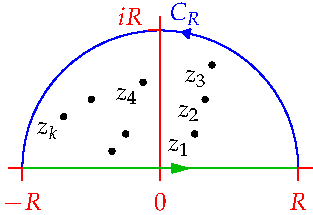
\includegraphics{integral}
\end{minipage}
\begin{enumerate}\setcounter{enumi}{2}
  \item If $\displaystyle\lim\limits_{R\to\infty}\int_{C_R}f(z)\,\dz=0$, then
$\displaystyle\text{P.V.}\int_{-\infty}^\infty f(x)\,\dx=2\pi i\sum\limits_{k=1}^n\Resl{z=z_k}f(z)$
\end{enumerate}

Mostly we will apply the method to rational functions $f(z)=\frac{p(z)}{q(z)}$, though it works more generally. Beyond ease of residue calculation, the reason is that $\deg q\ge \deg p+2$ is enough to guarantee that step 3 applies (Exercise \ref{exs:rationalimpint}).

\goodbreak


\begin{examples}{}{impexs}
\hangindent\leftmargini
\textup{1.} \ $f(z)=\frac 1{z^2+1}=\frac 1{(z-i)(z+i)}$ has simple poles at $\pm i$. Provided $\nm z=R>1$,
\begin{enumerate}\setcounter{enumi}{1}
  \begin{minipage}[t]{0.65\linewidth}\vspace{-10pt}
  \item[]\begin{gather*}
  \nm{z^2+1}\ge \nm{\nm z^2-1}=R^2-1\implies \frac 1{\nm{z^2+1}}\le\frac 1{R^2-1}\\
  \implies\nm{\oint_{C_R}f(z)\,\dz}\le \frac{\pi R}{R^2-1}\xrightarrow[R\to\infty]{}0\\
  \implies \,\text{P.V.}\int_{-\infty}^\infty\frac 1{x^2+1}\,\dx=2\pi i\Resl{z=i}f(z)=\frac{2\pi i}{2i}=\pi
  \end{gather*}
  Compare with the usual calculus method:
  \[\int_{-\infty}^\infty \frac 1{x^2+1}\,\dx=\tan^{-1}x\Big|_{-R_1\to-\infty}^{R_2\to\infty}=\pi\]
	\end{minipage}\begin{minipage}[t]{0.35\linewidth}\vspace{0pt}
	\flushright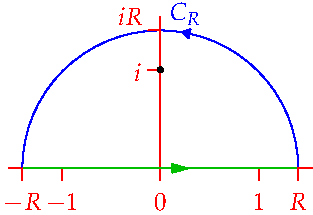
\includegraphics{integral2}
	\end{minipage}\par
  
  
  \begin{minipage}[t]{0.65\linewidth}\vspace{0pt}
	\item $f(z)=\frac{4(z^2-1)}{z^4+16}$ has simple poles at $\pm 2\zeta,\pm 2\zeta^3$ where $\zeta=\polar{\pi i}4$.\par
	Let $p(z)=16(z^2-1)$ and $q(z)=z^4+16$, so that
  \[\Res\limits_{z=z_0}f(z)=\frac{p(z_0)}{q'(z_0)}=\frac{z_0^2-1}{z_0^3}\]
	When $\nm z=R>2$, we see that
	\end{minipage}\begin{minipage}[t]{0.35\linewidth}\vspace{0pt}
	\flushright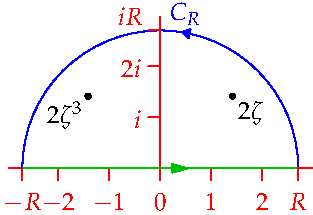
\includegraphics{integral3}
	\end{minipage}\par\vspace{-5pt}
  \begin{gather*}
  \nm{z^4+16}\ge R^4-16\implies \nm{\oint_{C_R}f(z)\,\dz}\le\frac{4\pi R(R^2+1)}{R^4-16}\to 0\\
  \text{P.V.\ }\int_{-\infty}^\infty f(x)\,\dx =2\pi i\left(\Resl{z=2\zeta}f(z)+\Resl{z=2\zeta^3}f(z)\right) =2\pi i\left(\frac{4\zeta^2-1}{8\zeta^3}+\frac{4\zeta^6-1}{8\zeta^9}\right) =\frac{3\pi}{2\sqrt 2}%\\
  %&=\frac{2\pi i}\zeta\left(\frac 48-\frac 1{8i}+\frac 4{8i}-\frac 18\right) =\frac{2\pi i\sqrt 2}{1+i}\cdot \frac 38(1-i) =\frac{3\pi}{2\sqrt 2}
  \end{gather*}
  

  \item\label{ex:smallarc} Variations are possible, for instance by taking only part of a semi-circular arc. The function $f(z)=\frac 1{z^5+1}$ has five simple poles: the fifth-roots of $-1$.\par
 	\begin{minipage}[t]{0.65\linewidth}\vspace{-10pt}
Since the pole $\zeta\omega^2=-1$ lies on the negative real axis, the integral $\int_{-\infty}^\infty f(x)\,\dx$ diverges. Instead consider the arcs in the picture when $R>1$. Parametrizing $C_2$ via $z(t)=t\omega$,
\begin{align*}
\int_{\textcolor{purple}{C_2}}\frac 1{z^5+1}\,\dz&= \int_R^0\frac{\omega}{t^5+1}\,\dt=-\omega\int_0^R\frac{1}{t^5+1}\,\dt\\
&=-\omega\int_{\textcolor{Green}{C_1}}\frac 1{z^5+1}\,\dz
\end{align*}
\end{minipage}\begin{minipage}[t]{0.35\linewidth}\vspace{-25pt}
\flushright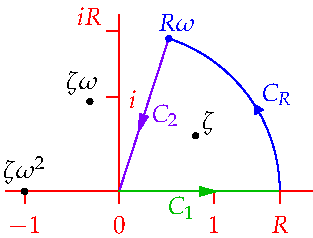
\includegraphics{integral4}
\end{minipage}\par\vspace{-5pt}
\[\implies(1-\omega)\int_0^R\frac 1{x^5+1}\,\dx+\int_{\textcolor{blue}{C_R}}\frac 1{z^5+1}\,\dz=2\pi i\Res_{z=\zeta}\frac 1{z^5+1} =\frac{2\pi i}{5\zeta^4}=\frac{2\pi i}{5\omega^2}\]
When $\nm z=R>1$, we see that $\nm{z^5+1}\ge R^5-1\implies\nm{\int_{C_R}\frac 1{z^5+1}\,\dz}\le\frac{2\pi R}{5(R^5-1)}\xrightarrow[R\to\infty]{}0$, and we conclude
\[\int_0^\infty\frac 1{x^5+1}\,\dx=\frac{2\pi i}{5(\omega^2-\omega^3)} =\frac{2\pi i}{5\zeta\omega^2(\zeta^{-1}-\zeta)} =\frac{2\pi i}{5(2i\sin\frac\pi 5)}=\frac \pi 5\csc\frac\pi 5\]
\end{enumerate}
\end{examples}



\boldsubsubsection{Jordan's Lemma}

It is often useful, particularly when computing Fourier transforms,\footnote{The Fourier transform of $f(x)$ is the function $\hat f(\xi):=\int_{-\infty}^\infty f(x)e^{-2\pi ix\xi}\,\dx$.} to evaluate integrals of the form
\[\int_{-\infty}^\infty f(x)e^{iax}\,\dx=\int_{-\infty}^\infty f(x)\cos ax\,\dx+i\int_{-\infty}^\infty f(x)\sin ax\,\dx\]
where $a>0$ is a real constant and $f:\R\to\C$ is a given function. If $f(x)$ is real-valued, then the above breaks the integral into real and imaginary parts. Given reasonable conditions on $f(x)$, the above method can often be employed.

\begin{example}{}{}
The function $f(z)=\frac{e^{3iz}}{z^2+4}$ is analytic on the upper half-plane except at the simple pole $z=2i$. With $R>2$ and $C_R$ the usual semi-circle, we see that
\begin{gather*}
\nm{e^{3iz}}=e^{-3y}\le 1\implies \nm{\int_{C_R}f(z)e^{3iz}\,\dz}\le \frac{\pi R}{R^2-4}\xrightarrow[R\to\infty]{} 0\\
\implies \text{P.V.}\int_{-\infty}^\infty \frac{e^{3ix}}{x^2+4}\,\dx =\lim_{R\to\infty}\int_{-R}^R \frac{e^{3ix}}{x^2+4}\,\dx =2\pi i\Res_{z=2i}\frac{e^{3iz}}{z^2+4} =2\pi i\frac{e^{-6}}{4i} =\frac 12\pi e^{-6}
\end{gather*}
Since this is real, we see that the result is in fact the integral $\int_{-\infty}^\infty \frac{\cos 3x}{x^2+4}\,\dx$. We don't need the Cauchy principal value of the integral here since the full improper integral converges. The corresponding imaginary integral is trivially zero since $\frac{\sin x}{x^2+1}$ is an odd function.
\end{example}

To assist with these computations, we state the following result without proof.

\begin{thm}{Jordan's Lemma}{}
Let $a,R_0>0$ be given and suppose $f(z)$ is analytic at all points exterior to $C_{R_0}$ in the upper half-plane. Suppose also that
\[\forall R>R_0,\ \exists M_R\text{ such that }\nm{f(z)}\le M_R\text{ and }\lim_{R\to\infty}M_R=0\]
Then $\lim\limits_{R\to\infty}\int_{C_R}f(z)e^{iaz}\,\dz=0$. If $f(z)$ also satisfies the hypotheses of our method, then
\[\text{P.V.}\int_{-\infty}^\infty f(x)e^{iax}\,\dx=2\pi i\sum_{j=1}^k\Res_{z=z_j}f(z)e^{iaz}\]
\end{thm}

\begin{example}{}{}
If $f(x)=\frac{x+1}{x^2+9}$ and $R>3$, then
\begin{gather*}
\nm{f(z)}=\frac{\nm{z+2}}{\nm{z^2+9}}\le\frac{R+2}{R^2-9} =M_R\xrightarrow[R\to\infty]{}0\\
\implies \text{P.V.}\int_{-\infty}^\infty\frac{(x+2)e^{iax}}{x^2+9}\,\dx=2\pi i\Res_{z=3i}\frac{(z+2)e^{iaz}}{z^2+9}=\frac{2\pi i(2+3i)e^{-3a}}{6i} =\frac{\pi(2+3i)}3e^{-3a}
\end{gather*}
By considering even and odd functions, etc., we can rewrite this as
\[\int_0^\infty\frac{\cos ax}{x^2+9}\,\dx =\frac{\pi}{6}e^{-3a}\qquad \int_0^\infty\frac{x\sin ax}{x^2+9}\,\dx =\frac{\pi}{2}e^{-3a}\]
\end{example}

\boldinline{Indented paths}

Another modification allows $f(z)$ to have a simple pole on the real axis.

\begin{lemm}[lower separated=false, sidebyside, sidebyside align=top seam, sidebyside gap=0pt, righthand width=0.3\linewidth]{}{simppoleint}
Let $D$ be the disk $\nm{z-z_0}\le\epsilon$, let $\delta<\epsilon$, and let $C_\delta$ be the clockwise semi-circle in the picture.
\begin{enumerate}
  \item If $\phi(z)$ is analytic on $D$, then $\lim\limits_{\delta\to 0}\int_{C_\delta}\phi(z)\,\dz=0$.
  \item If $f(z)$ is analytic on $D\setminus\{z_0\}$ with a simple pole at $z_0$, then
  \[\lim_{\delta\to 0}\int_{C_\delta}f(z)\,\dz=-\pi i\Res_{z=z_0}f(z)\] 
\end{enumerate}
\tcblower
\flushright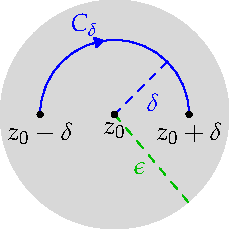
\includegraphics{integral5}
\end{lemm}

More generally, if $C_\delta$ spans $\theta$ radians clockwise round $z_0$, then $\lim\limits_{\delta\to 0}\int_{C_\delta}f(z)\,\dz=-i\theta\Res\limits_{z=z_0}f(z)$.

\begin{proof}
\begin{enumerate}
  \item $\phi$ is continuous on $D$ and thus bounded by some $M$: but then
	\[\nm{\int_{C_\delta}\phi(z)\,\dz}\le M\pi \delta\]
	\item The Laurent series expansion of $f(z)$ on $D\setminus\{z_0\}$ is
	\[f(z)=\frac{a_{-1}}{z-z_0}+\phi(z)\]
	where $a_{-1}=\Res\limits_{z=z_0}f(z)$ and $\phi(z)$ is analytic on $D$. Now evaluate
	\[\int_{C_\delta}\frac{a_{-1}}{z-z_0}\,\dz=a_{-1}\int_{\pi}^0\frac 1{\delta e^{i\theta}}i\delta e^{i\theta}\,\dth =- ia_{-1}\int_{0}^\pi\,\dth=-\pi ia_{-1}\tag*{\qedhere}\]
\end{enumerate}
\end{proof}

\begin{example}{}{}
Consider $f(z)=\frac{e^{iz}}z$. If $0<\delta<R$, then
\[\left(\int_{-R}^{-\delta}+\int_\delta^R\right)f(x)\,\dx=\left(\int_{-R}^{-\delta}+\int_\delta^R\right)\frac{\cos x+i\sin x}{x}\,\dx =2i\int_\delta^R\frac{\sin x}x\,\dx\]

\begin{minipage}[t]{0.59\linewidth}\vspace{0pt}
by even/oddness. Moreover, by Lemma \ref{lemm:simppoleint},
\[\lim_{\delta\to 0}\int_{C_\delta}\frac{e^{iz}}z\,\dz=-i\pi\Res_{z=0}f(z)=-i\pi\]
Since $\nm{f(z)}=\frac{e^{-y}}R\le \frac 1R$ on $C_R$, Jordan's lemma tells us that
\[0=2i\int_0^\infty\frac{\sin x}x\,\dx-i\pi\implies \int_0^\infty\frac{\sin x}x\,\dx=\frac\pi 2\]
\end{minipage}
\begin{minipage}[t]{0.4\linewidth}\vspace{0pt}
\flushright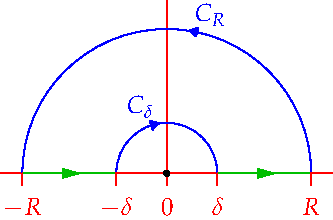
\includegraphics{integral6}
\end{minipage}
\end{example}

The example relied on the evenness of $\frac{\sin x}x$ and on the fact that the region of the half-plane between $C_R$ and $C_\delta$ contains no poles of $f(z)$. We essentially evaluated $\int_0^R\frac{\sin x}x\,\dx=\frac 12\int_{-R}^R\frac{\sin x}x\,\dx$ using an \emph{indented path} lying on the $x$-axis but dodging round the simple pole at zero. Many other versions of this trick are possible!


\begin{exercises*}
\hangindent\leftmargini
Many of these problems require extensive calculation to evaluate using residues: take your time and use it as an excuse to practice the previous section.

\begin{enumerate}
  \item Use residues to verify the values of the improper integrals:
  \begin{enumerate}
    \item $\displaystyle\int_0^\infty\frac{\dx}{(x^2+1)^2}=\frac\pi 4$\qquad
    (b)\ \ $\displaystyle\int_0^\infty\frac{x^2\,\dx}{x^6+1}=\frac\pi 6$
    
    \item[(c)] $\displaystyle\int_0^\infty\frac{x^2\,\dx}{(x^2+1)(x^2+4)}=\frac\pi 6$\qquad
    (d)\ \ $\displaystyle\int_0^\infty\frac{x^2\,\dx}{(x^2+9)(x^2+4)^2}=\frac\pi{200}$
  \end{enumerate}
  
  \item Find the Cauchy principal value of the integrals:
  \begin{enumerate}
    \item $\displaystyle\int_{-\infty}^\infty\frac{\dx}{x^2+2x+2}$\qquad
    (b)\ \ $\displaystyle\int_{-\infty}^\infty\frac{x\dx}{(x^2+1)(x^2+2x+2)}$
  \end{enumerate}
  
  \item Let $m,n$ be integers where $0\le m\le n-2$. By mimicking Example \hyperref[ex:smallarc]{\ref*{ex:impexs}.\ref*{ex:smallarc}}, prove that
  \[\int_0^\infty\frac{x^m}{x^n+1}\,\dx=\frac\pi n\csc\frac{(m+1)\pi}n\]  
  
  \item\begin{enumerate}
    \item If $\int_{-\infty}^\infty f(x)\,\dx$ converges, prove that it equals its Cauchy principal value.
    
    \item Suppose $f(x)$ is an even function and that $\text{P.V.}\int_{-\infty}^\infty f(x)\,\dx$ exists. Prove that $\int_{-\infty}^\infty f(x)\,\dx$ exists and has the same value.
  \end{enumerate}
  
  \item\label{exs:rationalimpint} If $f(x)=\frac{p(x)}{q(x)}$ is a rational function where $q(x)$ has no zeros and where $2+\deg p\le\deg q$, prove that $\int_0^\infty f(x)\,\dx$ converges.\par
    (\emph{Hint: let $p,q$ be monic and recall the comparison test for improper integrals})


	

	
  \item Prove the integration formulae:
  \begin{enumerate}
    \item $\displaystyle\int_{-\infty}^\infty \frac{\cos x\,\dx}{(x^2+a^2)(x^2+b^2)} =\frac\pi{a^2-b^2}\left(\frac{e^{-b}}b-\frac{e^{-a}}a\right)$ \ if $a>b>0$
    
    %\item $\displaystyle\int_{0}^\infty \frac{\cos ax\,\dx}{x^2+1} =\frac\pi 2e^{-a}$ if $a>0$
    
    \item $\displaystyle\int_{0}^\infty \frac{\cos ax\,\dx}{(x^2+b^2)^2} =\frac\pi{4b^3}(1+ab)e^{-ab}$ \ if $a,b>0$
    
    %\item $\displaystyle\int_{-\infty}^\infty \frac{x\sin ax\,\dx}{x^4+4} =\frac\pi 2e^{-a}\sin a$ if $a>0$
	\end{enumerate}
	
	\item Evaluate the integrals:
  \begin{enumerate}
    \item $\displaystyle\int_{-\infty}^\infty \frac{x\sin x\,\dx}{(x^2+1)(x^2+4)}$\qquad (b)\ \ $\displaystyle\int_{0}^\infty \frac{x^3\sin x\,\dx}{(x^2+1)(x^2+9)}$
	\end{enumerate}
	
	\item If $a$ is any real number and $b>0$, find the Cauchy principal value of $\displaystyle\int_{-\infty}^\infty\frac{\cos x\,\dx}{(x+a)^2+b^2}$
	
	\item Use the function $f(z)=z^{-2}(e^{iaz}-e^{ibz})$ and an indented contour around $z_0=0$ to prove that
	\[\int_0^\infty \frac{\cos ax-\cos bx}{x^2} =\frac\pi 2(b-a)\quad a,b\ge 0\]
	
	\item By integrating the function $f(z)=\frac{z^{-1/2}}{z^2+1}=\frac{\exp(-\frac 12\log z)}{z^2+1}$ where $\arg z\in(-\frac\pi 2,\frac{3\pi}2)$ along an indented contour, prove that
	\[\int_0^\infty \frac{\dx}{\sqrt x(x^2+1)} =\frac\pi{\sqrt 2}\]
  
  \item What happens to part 2 of Lemma \ref{lemm:simppoleint} if $f(z)$ is analytic on $D\setminus\{z_0\}$ but has a pole of order $m\ge 2$ at $z_0$.
  
  

	\item (Hard)\quad A similar trick can be applied with sequences of boundary curves $C_N$. For instance, for each $N\in\N$, let $C_N$ denote the positively oriented boundary of the square whose edges lie along the lines $x,y=\pm\left(N+\frac 12\right)\pi$. Prove that
  \[\oint_{C_N}\frac{\dz}{z^2\sin z}=2\pi i\left[\frac 16+2\sum_{n=1}^N\frac{(-1)^n}{n^2\pi^2}\right]\]
  Hence conclude that $\sum\limits_{n=1}^\infty\frac{(-1)^{n-1}}{n^2}=\frac{\pi^2}{12}$
\end{enumerate}
\end{exercises*}
